%
% mannigfaltigkeit.tex -- Mannigfaltigkeit
%
% (c) 2021 Prof Dr Andreas Müller, OST Ostschweizer Fachhochschule
%
\bgroup
\begin{frame}[t]
\setlength{\abovedisplayskip}{5pt}
\setlength{\belowdisplayskip}{5pt}
\frametitle{Mannigfaltigkeit}
\vspace{-20pt}
\begin{columns}[t,onlytextwidth]
\begin{column}{0.48\textwidth}
\begin{center}
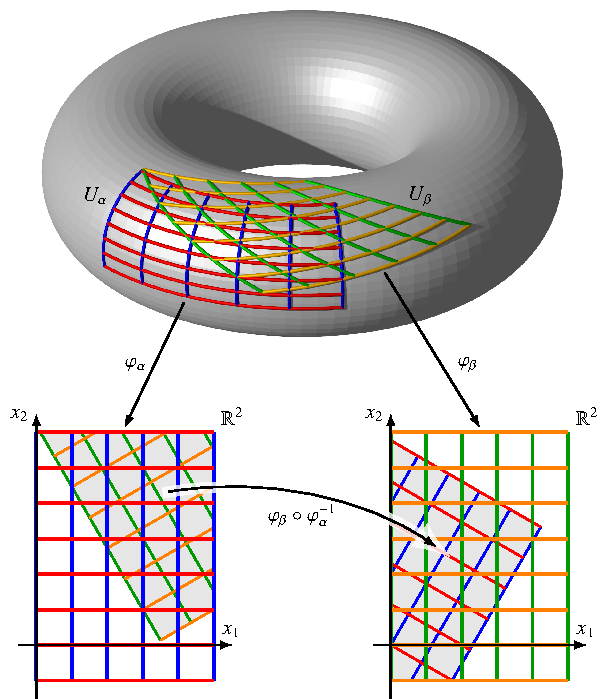
\includegraphics[width=\textwidth]{../../buch/chapters/60-gruppen/images/karten.pdf}
\end{center}
\end{column}
\begin{column}{0.48\textwidth}
\begin{block}{Definition}
\begin{itemize}
\item<2-> Karte: Abbildung $\varphi_\alpha\colon U_\alpha\to\mathbb{R}^n$
\item<3-> differenzierbare Kartenwechsel: Koordinatenumrechnung im Überschneidungsgebiet
\[
\varphi_\beta\circ\varphi_\alpha^{-1}
\colon
\varphi_\alpha(U_\alpha\cap U_\beta)
\to
\varphi_\beta(U_\alpha\cap U_\beta)
\]
\item<4-> Atlas: Menge von Karten, die die ganze Mannigfaltigkeit überdecken
\end{itemize}
\end{block}
\vspace{-7pt}
\uncover<5->{%
\begin{block}{Lokal$\mathstrut\cong\mathbb{R}^n$}
Differenzierbare Mannigfaltigkeiten sehen lokal wie $\mathbb{R}^n$ aus
\end{block}}
\vspace{-3pt}
\uncover<6->{%
\begin{block}{Lie-Gruppe}
Gruppe und Mannigfaltigkeit
\end{block}}
\end{column}
\end{columns}
\end{frame}
\egroup
